%************************************************
\chapter{Introduction}\label{ch:introduction}
%************************************************
Data from the World Economic Outlook, of the IMF (2013), list currently Brazil as the seventh largest economy in the world, with a GDP of US\$ 2,396 trillions. According to a survey by The Economist (2013), since 2009, the growth of BRICS (emerging market economies group formed by Brazil, Russia, India, China and South Africa) accounts for 55\% of the world economy growth. The current economic scenario is extremely favorable for Brazil to increase its global influence.

However, with regard to the ability to communicate globally, we occupy a much more modest position. In the \ac{EF-EPI} of 2014, which is published by \ac{EF}, Brazil was ranked in the 38\textsuperscript{th} position out of 63 countries, classified among countries with low English proficiency, with $49.96$ points \cite{EF2014}. The full ranking is shown in \autoref{fig:ef-epi-ranking}.

\begin{figure}[!htpb]
  \centering
  {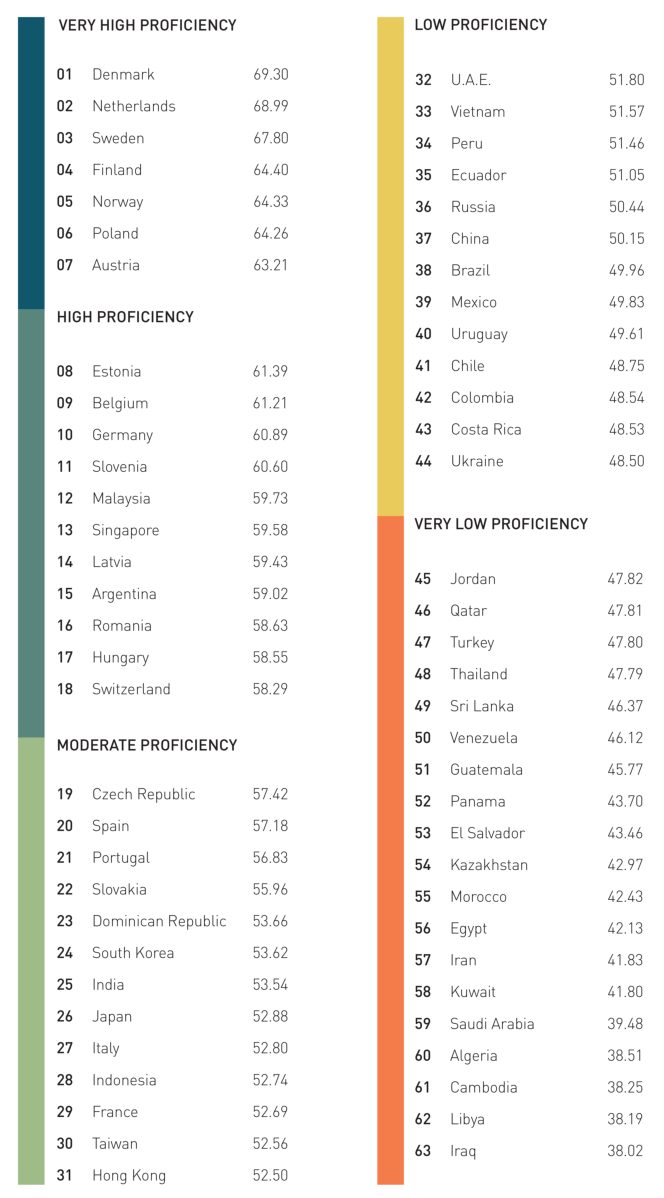
\includegraphics[width=0.7\linewidth]{gfx/ef-epi-ranking-2014.pdf}}
  \caption{English Proficiency Index 2014 Rankings \cite{EF2014}.}
  \label{fig:ef-epi-ranking}
\end{figure}

As can be noticed from \autoref{fig:ef-epi-ranking}, Brazil was immediately behind two other countries from the BRICS, Russia ($50.44$) and China ($50.15$); and near several other Latin America countries, such as Peru ($51.46$), Ecuador ($51.05$), Uruguay ($49.61$), Chile ($48.75$) and Colombia ($48.54$). 

Scandinavian countries lead the very high proficiency rankings, with Denmark ($69.30$) in the first position, Sweden ($67.30$) in third the spot, Finland ($64.40$) in the fourth and Norway ($64.33$) in the fifth. All these countries have a very high \ac{HDI}, according to the United Nations Development Programme. The \ac{HDI} measures the social and economic development by analyzing three indexes: educational level, average income and longevity. The top five in the \ac{EF-EPI} rankings are among the top twelve countries in terms of \ac{HDI} \cite{HDI2014}. The \ac{EF-EPI} data showed that there is a moderate to strong correlation between \ac{HDI} and English proficiency (R=0.67) \cite{EF2014}. The second position in the \ac{EF-EPI} ranking is held by the Netherlands, scoring $68.99$ points. The Netherlands has the fourth largest \ac{HDI} in the world. This result is similar to that of the previous versions of \ac{EF-EPI} \cite{EF2013, EF2012, EF2011}, which also showed a prevalence of Northern European countries in the best positions.

It is interesting to notice that four of the countries at the top five share a common cultural Germanic heritage and speak a language of the Germanic family -- the same branch that English is part of. Since Danish, Swedish, Norse, Dutch and English are related through descent from a common ancestor, Proto-Germanic, they inevitably share many linguistic characteristics, such as sound correspondences, a large number of cognates, as well as similar morphology and syntax. This might be an advantage of these countries in comparison to the remaining.

The high proficiency band is occupied mainly by other European countries, both in the Eastern and Western part, such as Estonia (61.39), Belgium (61.21), Germany (60.89), Slovenia (60.60), Latvia (59.43) and Switzerland (58.29). Two Southeast Asian countries also figure within this range, namely Malaysia (59.73) and Singapore (59.58). This result might seem a bit biased since English is one of the official languages in Singapore, along with Malay, Mandarin and Tamil; it is considered the language of business, government, and the medium of instruction in school. We shall highlight Argentina's performance. Despite the great economic depression from 1998 to 2002, Argentina was still able to outperform Brazil, scoring $59.02$ points, being the only country from Latin America among the ones with high proficiency. 

The moderate proficiency range is filled by the remaining European countries, such as Czech Republic (57.42), Slovakia (55.96), the countries from the Iberian Peninsula -- Spain (57.18) and Portugal (56.83)--, together with France (52.69) and Italy (52.80). In addition, the majority of Asian countries which were analyzed in the survey also figure in this list. South Korea achieved the best performance among them, with 53.62 points. India comes next, scoring 53.54 points. The rest of the list is occupied by Japan (52.88), Indonesia (52.74), Taiwan (52.56) and Hong Kong (52.50).

The \ac{EF-EPI} bands are aligned to the \ac{CEFR}, which is a guideline proposed by the Council of Europe to describe achievements of learners of foreign languages across the European Union. The \ac{CEFR} reference levels are described in \autoref{tab:cefr-levels}. \ac{EF-EPI} bands are mapped into \ac{CEFR} reference levels as follows: the very high proficiency band corresponds to \ac{CEFR} level B2; very low proficiency to A2; high, moderate and low proficiency bands to B1 with different punctuations. 

\begin{table}[!htpb]
\newcolumntype{A}{>{\centering\arraybackslash}m{.12\textwidth}}
\newcolumntype{B}{>{\centering\arraybackslash}m{.12\textwidth}}
\newcolumntype{C}{>{\arraybackslash}m{.64\textwidth}}
\caption{CEFR reference levels.}
\scriptsize
\begin{center}
\begin{tabular}{ABC}
\hline
\textbf{ Group} & \textbf{Level} & \textbf{\centering Description} \\ \hline
\multicolumn{ 1}{A}{\textbf{Basic User
(A)}} & \multicolumn{ 1}{B}{\textbf{Beginner (A1)}} & Can understand and use familiar everyday expressions and very basic phrases aimed at the satisfaction of needs of a concrete type. \\ 
\multicolumn{ 1}{A}{} & \multicolumn{ 1}{B}{} & Can introduce him/herself and others and can ask and answer questions about personal details such as where he/she lives, people he/she knows and things he/she has. \\ 
\multicolumn{ 1}{A}{} & \multicolumn{ 1}{B}{} & Can interact in a simple way provided the other person talks slowly and clearly and is prepared to help. \\ \cline{ 2- 3}
\multicolumn{ 1}{A}{} & \multicolumn{ 1}{B}{\textbf{Elementary (A2)}} & Can understand sentences and frequently used expressions related to areas of most immediate relevance (e.g. very basic personal and family information, shopping, local geography, employment). \\ 
\multicolumn{ 1}{A}{} & \multicolumn{ 1}{B}{} & Can communicate in simple and routine tasks requiring a simple and direct exchange of information on familiar and routine matters. \\ 
\multicolumn{ 1}{A}{} & \multicolumn{ 1}{B}{} & Can describe in simple terms aspects of his/her background, immediate environment and matters in areas of immediate need. \\ \hline
\multicolumn{ 1}{A}{\textbf{Independent User 
(B)}} & \multicolumn{1}{B}{\textbf{Intermediate (B1)}} & Can understand the main points of clear standard input on familiar matters regularly encountered in work, school, leisure, etc. \\ 
\multicolumn{ 1}{A}{} & \multicolumn{ 1}{B}{} & Can deal with most situations likely to arise while traveling in an area where the language is spoken. \\ 
\multicolumn{ 1}{A}{} & \multicolumn{ 1}{B}{} & Can produce simple connected text on topics that are familiar or of personal interest. \\
\multicolumn{ 1}{A}{} & \multicolumn{ 1}{B}{} & Can describe experiences and events, dreams, hopes and ambitions and briefly give reasons and explanations for opinions and plans. \\ \cline{ 2- 3}
\multicolumn{ 1}{A}{} & \multicolumn{ 1}{B}{\textbf{Upper intermediate (B2)}} & Can understand the main ideas of complex text on both concrete and abstract topics, including technical discussions in his/her field of specialization. \\ 
\multicolumn{ 1}{A}{} & \multicolumn{ 1}{B}{} & Can interact with a degree of fluency and spontaneity that makes regular interaction with native speakers quite possible without strain for either party. \\ 
\multicolumn{ 1}{A}{} & \multicolumn{ 1}{B}{} & Can produce clear, detailed text on a wide range of subjects and explain a viewpoint on a topical issue giving the advantages and disadvantages of various options. \\ \hline
\multicolumn{ 1}{A}{\textbf{Proficient User
(C)}} & \multicolumn{ 1}{B}{\textbf{Advanced (C1)}} & Can understand a wide range of demanding, longer texts, and recognize implicit meaning. \\ 
\multicolumn{ 1}{A}{} & \multicolumn{ 1}{B}{} & Can express ideas fluently and spontaneously without much obvious searching for express \\ 
\multicolumn{ 1}{A}{} & \multicolumn{ 1}{B}{} & Can use language flexibly and effectively for social, academic and professional purposes. \\ 
\multicolumn{ 1}{A}{} & \multicolumn{ 1}{B}{} & Can produce clear, well-structured, detailed text on complex subjects, showing controlled use of organizational patterns, connectors and cohesive devices. \\ \cline{ 2- 3}
\multicolumn{ 1}{A}{} & \multicolumn{ 1}{B}{\textbf{Proficiency (C2)}} & Can understand with ease virtually everything heard or read. \\ 
\multicolumn{ 1}{A}{} & \multicolumn{ 1}{B}{} & Can summarize information from different spoken and written sources, reconstructing arguments and accounts in a coherent presentation. \\ 
\multicolumn{ 1}{B}{} & \multicolumn{ 1}{B}{} & Can express him/herself spontaneously, very fluently and precisely, differentiating finer shades of meaning even in the most complex situations. \\ \hline
\end{tabular}
\end{center}
\label{tab:cefr-levels}
\end{table}

In case, Brazil's low proficiency rank is analogous to the \ac{CEFR} B1 level. To put another way, it means that Brazilians are usually able to communicate in English with intermediate skills, being able to understand familiar matters, deal with traveling situations, describe personal experiences and plans, and produce simple texts about subjects of personal interest. As one might observe this is a very restricted communicative competence, which limits English usage basically to the personal domain. To get an idea, the \ac{CEFR} lists four broad domains: educational, occupational, public, and personal. So Brazilians lacks linguistic abilities in at least three broad domains, this linguistic competence would not allow one to perceive or produce English utterances flexibly, either for social, academic or professional purposes. The performance for each state can be found at the map in \autoref{fig:ef-epi-brazil-map}.

\begin{figure}[!ht]
  \centering
  {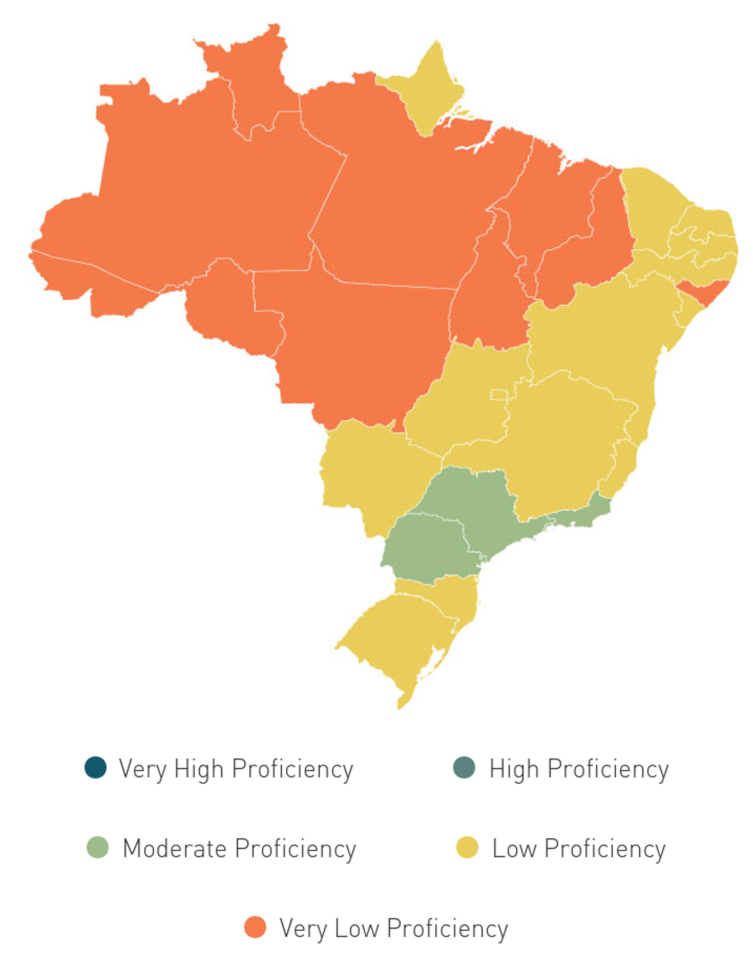
\includegraphics[width=.6\linewidth]{gfx/ef-epi-brazil-map.pdf}}
  \caption{EF EPI scores for each Brazilian state.}
  \label{fig:ef-epi-brazil-map}
\end{figure}

As one might see from \autoref{fig:ef-epi-brazil-map}, one can clearly see division between Southern and Northern Brazil. Ten states achieved very low proficiency, namely Amazonas, Acre, Par\'a, Roraima, Piau\'i, Alagoas, Tocantins, Rond\^onia, Maranh\~ao and Mato Grosso. The highest scores are found among the richest Brazilian states, mainly in the Southeast and the South regions. The top position is held by S\~ao Paulo, which has the largest population, the highest number of industries, and most part of the economic production in the country. Rio de Janeiro, which is the second largest economy of Brazil, occupies the second position. Paran\'a is the third best ranked state. These three states are the only in the country that achieved moderate proficiency, they attained a score that is at least $4.8\%$ above the country's average, and all of them are among those with the highest \ac{HDI}.

With respect of Business English proficiency, our performance is even more concerning. On the 
2013 \ac{BEI}, conducted by \citeauthor{BEI2013} \cite{BEI2013}, Brazil reached the 71\textsuperscript{st} position out of 77 countries analyzed. Brazil attained a score of $3.27$ points, in a scale from $1$ to $10$, being placed at the ``Beginner'' range, the lowest proficiency range considered by the index. Brazil's performance was close to that of El Salvador ($3.24$), Saudi Arabia ($3.14$) and Honduras ($2.92$) which up until recently had experienced civil wars or dictatorship governments. The ``Beginner'' level is described as: ``Can read and communicate using only simple questions and statements, but can't communicate and understand basic business information during phone calls.'' Again, we can see that this is a very limited linguistic competence, that would not allow one not even to perform the most elementary day-to-day tasks in a company or industry work environment.

Given this scenario, it is clear that we desperately need to improve English language proficiency among Brazilians. This project seeks to be an initial step towards this direction. I developed several tools and resources for non-native speech recognition, focused on Brazilian-accented English or Brazilian Portuguese. In addition,  I created a prototype system for non-native speech recognition and correction, called Listener, which is capable of recognizing utterances in Brazilian-accented English and identifying which are the mispronunciations.

\section*{Contributions of the Thesis}

Within this work, I have investigated and developed a set of tools and resources for non-native speech recognition and correction, focused on Brazilian-accented English. Some of these resources and tools are exclusively for tasks related to processing Brazilian-accented English, but others can also be employed for many other purposes, such as a \ac{G2P} for \ac{BP} and balancing of speech corpus. The full list of contributions is provided below:

\begin{enumerate}
 \item \emph{Aeiouad\^o G2P}: A grapheme-to-phoneme converter for \ac{BP} which uses a hybrid approach, based on both handcrafted rules and machine learning method, as decribed in \citeauthor{Mendonca2014} \cite{Mendonca2014}. \emph{Aeiouad\^o dictionary}: A large machine readable dictionary for \ac{BP}, compiled from a word list extracted from the Portuguese Wikipedia, which was preprocessed in order to filter loanwords, acronyms, scientific names and other spurious data, and then transcribed with Aeiouad\^o G2P).
 \item A phonetic speller for user-generated content in \ac{BP}, based on machine learning, which takes advantage of Aeiouad\^o G2P to group phonetically related words, as described in \citeauthor{Mendonca2015} \cite{Mendonca2015}; 
 \item A method for the extraction of phonetically rich sentences, i.e. sentences with a high variety of triphones distributed in a uniform fashion, which employs a greedy algorithm for comparing triphone distributions among sentences, as described in \citeauthor{Mendonca2014b} \cite{Mendonca2014b};
 \item A crowdsourced platform for speeding up the process of compiling and transcribing speech corpora;
 \item A set of rules for generating pronunciation hypothesis for Brazilian-accented English, considering nine types of mispronunciations, respectively: (i) syllable simplification; (ii) consonant change; (iii) deaspiration of voiceless plosives in initial or stressed positions; (iv) terminal devoicing in word-final obstruents; (v) delateralization and rounding of lateral liquids in final position; (vi) vocalization of final nasals; (vii) velar consonantal paragoge; (viii) vowel assimilation; (ix) interconsonantal epenthesis;
 \item \emph{Listener}:A prototype system for automatic speech recognition and evaluation of Brazilian-accented English, which makes use of forced alignment, \ac{HMM}/\ac{GMM} acoustic models, context free grammars and multipronunciation dictionaries;
\end{enumerate}

All files, resources and scripts developed are available at the project website\footnote{Due to copyright reasons, the corpora used for training the acoustic models cannot be made available.}: 
\begin{center}
 \url{http://nilc.icmc.usp.br/listener}
\end{center}

\section*{Thesis Structure}

This Master's thesis is organized in seven chapters. \label{ch:foundations} presents the theoretical fundations, with an introduction to phonetics and phonology, second language acquisition as well as automatic speech recognition. \autoref{ch:aieouado-g2p} presents th Aeiouad\^o's grapheme-to-phoneme converter and dictionary. \autoref{ch:speller} presents a use-case of Aeiouad\^o, namely a phonetic-speller which employs the transcriptions generated by the grapheme-to-phoneme converter. \autoref{ch:phonetically-rich} proposes a method for the extraction of phonetically-rich sentences. \autoref{ch:listener} describes a prototype system for non-native speech recognition and evaluation of Brazilian-accented English, which makes use of the tools and resources developed in this thesis. Finally in \autoref{ch:conclusions}, we present the overall conclusions, some limitations we found, together with the next steps for future work. A glossary can be found at the back of the thesis in order to help the reader with uncommon terms or specialized jargon.